\section{Signal Start Detection}
\label{sec:04_signalStartDetection}

The implemented \ac{TDOA} algorithms requires a smaller number of signal samples
at the start of the signal to circumvent multi-path propagated signals and reverberation.
In which extend the reflections distorts the delays between the samples
will be handled in forthcoming sections.

% Especially the result in \cref{subsubsec:03_phase} has shown that in fact, the
% accuracy of the direction predictor decreases when evaluated on later samples
% of the whistle signal.\todo{Maybe interpret this somewhere: give a reason
% why shit makes sense (e.g. maybe because more reflections of the signal will
% have reached the microphone)}
% Also according to the outcome of \cref{subsec:04_psnr}, the \ac{GCC}
% method performs best with frames near to the signal start. \todo[inline]{Get
% rid of some cross-references and/or write more about what happened in these
% chapters. (I don't remember what happened in 3.4 and 4.2.3 and jumping back and
% forth is annoying.)}

% There are some reasons why other methods were tested to find the signal start.
In order to find a good solution for a highly reliable, accurate but
computationally tractable start detection, different approaches were
tested profoundly.
For high temporal accuracy either the window must be small or is must
be shifted with small steps which both implicit a large number of evaluations.
The existing whistle detection algorithm of the HULKs presented in
\cref{subsec:03_whistleDetection} is computationally intensive and has a low
accuracy for small sample selection windows as shown in \label{subsec:04_whistleDetection}.
Therefore, the goal is to identify a simple algorithm for
the signal start detection which is one of the approaches in \Cref{subsec:03_signalStartDetection}.
Ideally, this algorithm should be adaptable to signals other than the whistle-sounds.

Hereinafter, the performance of each method methods is evaluated by
analyzing the number of index difference between algorithmically determined start index
and manually labelled start index.
As a benchmark, the prediction accuracy is evaluated on the eleven laboratory-measurements
of all five robots \cref{subsec:04_labMeasurements} to compare the signal start detection algorithms.
By the frame size of the \ac{FFT} being set to 256 samples for the
correlation methods, a start index error of at most 256 samples is
desired.
Therefore, a start index detection result is regarded as failure for errors
larger than 256 for the following sections.
Having eleven whistle-sounds recorded with five robots, a total number
of 55 measurements arise.
Taking into account that each robot has four microphones attached,
the overall number increase to 220 recorded signals on which the signal start detection
algorithms can be tested.
% -----------------------------------------------------------------------------------------------------

\subsection{Whistle Detection}
\label{subsec:04_whistleDetection}

First, the accuracy of the whistle detection which is already a part of the HULKs' framework
is evaluated in regard of the start index.
Here, the start index is defined as the first index of a frame in which the whistle detection
found a whistle.
With a frame size of 1024, the whistle detection algorithm fails for 81\si{\percent}
of the 220 measurements.
However, every error is in the range of 1024 samples which proves that the
approximate start of the whistle-sound is detected correctly.
With a smaller frame size of 256, the temporal accuracy is improved up to a small
failure rate of 9\si{\percent} but also introduces false positive detections.
With the results, one can say that the whistle detection is not sufficient
for the start detection or is at least not reliable as stand-alone solution.
Furthermore, this approach is limited to sounds in fixed and known frequency range.
%  failure rate of
% 9\si{\percent} in regard to every channel.
% In this work microphone data were saved as soon as the whistle detection module
% found a whistle-sound in the audio samples.
% Due to this implementation, the algorithm does never fail to detect the whistle
% Standing alone, the error is always in the range of \si{\pm1024} samples due to the
% set frame size of 1024 samples.
% With a smaller frame size of 256, the accuracy gets better with an error of
% 9\si{\percent} in regard to the 220 samples but has an error rate of
% 25.5\si{\percent} for the measurements.

% looking at the next 300
% values and with a step size of 50 the result is 15\si{\percent} and 36\si{\percent}
% and with step size 1, it is 13\si{\percent} and 33\si{\percent}.
% This is computationally very costly and the reward is small.

\subsection{ZCR}
\label{subsec:04_zcr}

For the evaluation of the \ac{ZCR},
the frame size is set to 256 samples and number of noise and signal frames
are set to 10 frames.
In 7\si{\percent} of the 220 channel samples, this method fails.
In most cases, the method provides accurate results with
small error. Taking all measurements of robot 26 as example, the \ac{RMSE}
amounts 77.06 samples.

\btline{H}{1.2}
\btab{|c|c|c|c|}
\hline
Measurement & ZCR Error & Entropy Error & WD Error\\
\hline
0 & 48.17 & 129.15 & 359.25\\
\hline
1 & 71.66 & 63.82 & 260.4\\
\hline
2 & 85.84 & 66.31 & 320.06\\
\hline
3 & 63.67 & 46.29 & 215.35\\
\hline
4 & 66.9 & 212.31 & 210.32\\
\hline
5 & 79.17 & 52.99 & 203.82\\
\hline
6 & 84.22 & 43.51 & 13064.78\\
\hline
7 & 78.2 & 54.27 & 290.59\\
\hline
8 & 86.06 & 149.29 & 118.02\\
\hline
9 & 88.24 & 199.33 & 140.38\\
\hline
10 & 95.54 & 290.02 & 202.32\\
\hline
\etab
\et{Comparison of the signal start detection methods with a frame size of 512 samples.
	Laboratory-measurements on robot no. 26 are selected
	to show the results exemplary. WD stands for whistle detection and the error are
	\acp{RMSE} between the channels}{04_ssdComparison}

However, there are cases where the algorithm fails. Looking at those cases it
could be identified that the errors occur often due to incorrect assumptions
that the signal is present at the end of the buffered samples.
Some measurements prove that this is not always the case as shown in
\cref{fig:04_zcrFail}.
The figure presents a case where the whistle signal ended around 35000 samples.
If the start index is determined at the point where the \ac{ZCR}
falls below the threshold searching backwards as stated in \cref{sec:02_signalStartDetection},
the detection fails.

In many cases, only one out of four channels produces an erroneous
result.
Because the final start index on one robot is set equal for all channel,
the failure can be compensated with a simple voting procedure.
% -------------------------------------------------------------
\begin{figure}[ht]
	\centering
	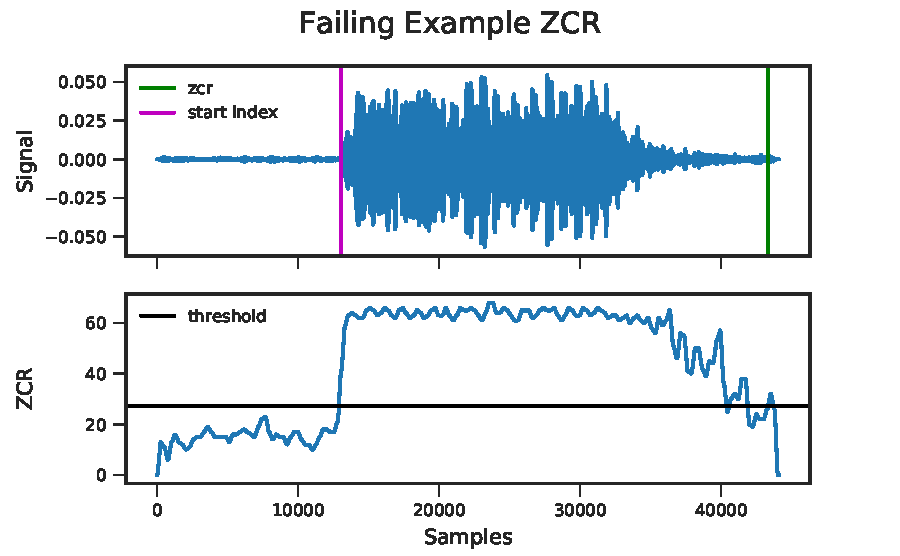
\includegraphics[]{figures/evaluation/zcr_fail}
	\caption{Channel 3 data from measurement 5 of \cref{subsec:04_labMeasurements}
		for robot number 21. A failing example for the start detection by \ac{ZCR}
		is shown.}
	\label{fig:04_zcrFail}
\end{figure}
% -------------------------------------------------------------
If the start index is determined at the point where the \ac{ZCR}
falls below the threshold searching backwards as stated in \cref{sec:02_signalStartDetection},
the detection fails.

% Another option exists by changing the process of finding the
% threshold excess onwards.\todo{I don't understand what this is saying.}
% In this case, the threshold is scaled with a factor of 1.25.
% Results by this were poorer than the initially implemented manner
% with a failure rate of 15\si{\percent}.\todo{Did you ever report the previous failure rate?}
% By adding the constraint that multiple samples must exceed the
% threshold successively, result can be slightly improved for the cost of higher
% computational effort.

% It should be noted that the poor performance of the \ac{ZCR} method with signal that
% was cleaned with spectral subtraction previously. This surprising outcome is
% convenient for the overall task, because the start index result can be embed
% into the spectral subtraction, providing information for separating the noise
% and signal part.\todo{I don't get what this paragraph is saying?}

\subsection{Entropy}
\label{subsec:04_entropy}

As discussed in \cref{subsec:02_Entropy} the entropy quantifies the amount
of disorder in a signal frame.
Especially for signals to localize with unknown characteristics,
this method can be useful because the only a-priori knowledge must be,
that the signal to detect has lower entropy than the background noise.
For all measurements this method yielded poorer results than the \ac{ZCR} method
with a failure rate of around 18\si{\percent}.
Best results are achieved with a frame size of 512 samples and a step size of 800
samples.
% \change[]{Explain what steps are? Maybe in implementation?}
However, for records where the whistle ends before the end of the recorded signal
it generates more reliable results than the \ac{ZCR} method.
Taking the same measurement as an example for which failure of the \ac{ZCR} method
was discussed earlier, \cref{fig:04_entropyGood} shows how the algorithm
detects the signal start correctly even though the whistle-sound ended at
around 35000 samples. In this measurement, the start index errors of all four
channels were smaller than 40 samples.
% -------------------------------------------------------------
\begin{figure}[ht]
	\centering
	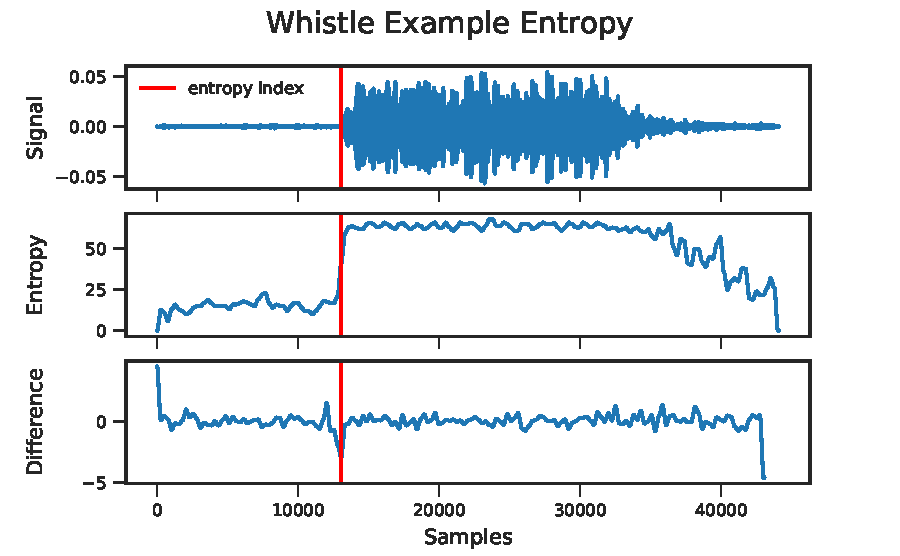
\includegraphics[]{figures/evaluation/entropy_good}
	\caption{Exemplary result of start index detection by entropy where
		the \ac{ZCR} method failed due to fading whistle
		at the data.}
	\label{fig:04_entropyGood}
\end{figure}
% -------------------------------------------------------------

% But as the entropy should be larger for noisy environment
% performance in other surrounding of measurement at \ac{RoboCup} is looked at.
% Entropy would be best for undefined signal -> distinguish between
% signal and noise without information